\documentclass[12pt]{article}

\usepackage[a4paper, margin=1in]{geometry}
\usepackage{graphicx}
\usepackage{amsmath}
\usepackage{booktabs}
\usepackage{caption}
\usepackage{listings}
\usepackage{xcolor}
\usepackage{hyperref}
\usepackage{array}

% Define colors and style for code listings
\definecolor{codegreen}{rgb}{0,0.6,0}
\definecolor{codegray}{rgb}{0.5,0.5,0.5}
\definecolor{codepurple}{rgb}{0.58,0,0.82}
\definecolor{backcolour}{rgb}{0.95,0.95,0.92}

\lstdefinestyle{mystyle}{
    backgroundcolor=\color{backcolour},
    commentstyle=\color{codegreen},
    keywordstyle=\color{magenta},
    numberstyle=\tiny\color{codegray},
    stringstyle=\color{codepurple},
    basicstyle=\ttfamily\footnotesize,
    breakatwhitespace=false,
    breaklines=true,
    captionpos=b,
    keepspaces=true,
    numbers=left,
    numbersep=5pt,
    showspaces=false,
    showstringspaces=false,
    showtabs=false,
    tabsize=2,
    literate={--}{{-{}-}}2,
    extendedchars=true
}
\lstset{style=mystyle}

\title{Reinforcement Learning Policy Evaluation in a Grid World}
\author{20251203377}
\date{\today}

\begin{document}
\maketitle

\section{Problem Setup}
We evaluate two policies within a discrete $5 \times 3$ grid world environment. The setup is defined as follows:
\begin{itemize}
    \item \textbf{Environment:} A grid of size $5 \times 3$. The start state is $(0,2)$, the goal state is $(2,2)$, and there are forbidden states at $\{(2,1), (1,2), (3,1)\}$.
    \item \textbf{Action Space:} The agent can choose from five actions: $(0,1)$ (down), $(1,0)$ (right), $(0,-1)$ (up), $(-1,0)$ (left), and $(0,0)$ (stay).
    \item \textbf{Reward Function:} The agent receives a reward of $R_{\text{target}}=+1$ for reaching the goal state, $R_{\text{forbidden}}=-1$ for attempting to enter a forbidden state, and $R_{\text{step}}=0$ for all other valid moves.
    \item \textbf{Discount Rate:} Future rewards are discounted by a factor of $\gamma=0.9$.
\end{itemize}

\section{Policy 1: Deterministic Policy}
The first policy is deterministic and optimal, generated by a reverse Breadth-First Search (BFS) from the goal state. For any given state, this policy selects the action that moves the agent along a shortest path to the target.

\subsection{Policy Visualization}
The policy is visualized in Figure~\ref{fig:det_policy}, where arrows indicate the deterministic action for each state.

\begin{figure}[h!]
\centering
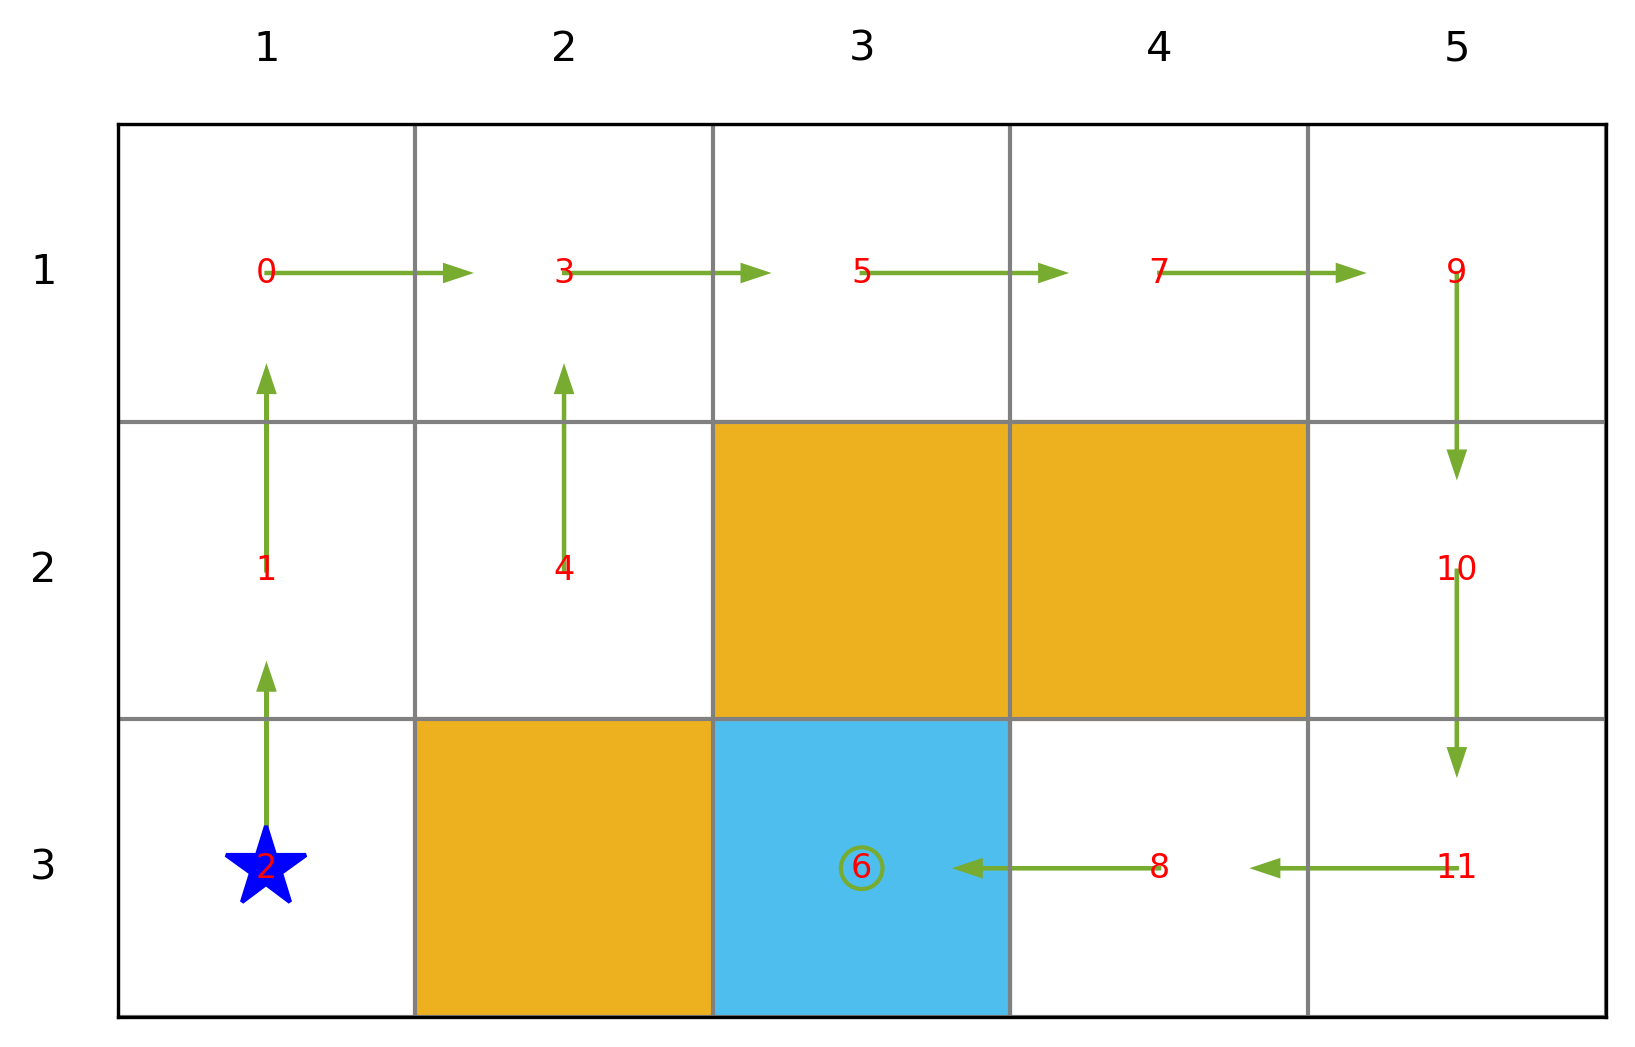
\includegraphics[width=0.8\textwidth]{output/deterministic_policy.png}
\caption{Deterministic policy visualized with arrows on the grid.}
\label{fig:det_policy}
\end{figure}

\subsection{Policy Dynamics: \texorpdfstring{$r^\pi$}{r pi} and \texorpdfstring{$P^\pi$}{P pi}}
The policy's expected one-step rewards, $r^\pi$, and state transition probabilities, $P^\pi$, are shown below.

\noindent\textbf{Reward Vector $r^\pi$:}

% Add a table to show the reward vector with state labels
\begin{center}
\begin{tabular}{|c|c|c|c|c|c|c|c|c|c|c|c|c|}
\hline
\textbf{State} & S0 & S1 & S2 & S3 & S4 & S5 & S6 & S7 & S8 & S9 & S10 & S11 \\
\hline
\textbf{Reward} & 0.0 & 0.0 & 0.0 & 0.0 & 0.0 & 0.0 & 1.0 & 0.0 & 1.0 & 0.0 & 0.0 & 0.0 \\
\hline
\end{tabular}
\end{center}

\noindent\textbf{Transition Matrix $P^\pi$:}

% Add a table to show the transition matrix with row and column labels
\begin{center}
\begin{tabular}{|c|c|c|c|c|c|c|c|c|c|c|c|c|c|}
\hline
\textbf{From/To} & \textbf{S0} & \textbf{S1} & \textbf{S2} & \textbf{S3} & \textbf{S4} & \textbf{S5} & \textbf{S6} & \textbf{S7} & \textbf{S8} & \textbf{S9} & \textbf{S10} & \textbf{S11} \\
\hline
\textbf{S0} & 0.0 & 0.0 & 0.0 & 1.0 & 0.0 & 0.0 & 0.0 & 0.0 & 0.0 & 0.0 & 0.0 & 0.0 \\
\hline
\textbf{S1} & 1.0 & 0.0 & 0.0 & 0.0 & 0.0 & 0.0 & 0.0 & 0.0 & 0.0 & 0.0 & 0.0 & 0.0 \\
\hline
\textbf{S2} & 0.0 & 1.0 & 0.0 & 0.0 & 0.0 & 0.0 & 0.0 & 0.0 & 0.0 & 0.0 & 0.0 & 0.0 \\
\hline
\textbf{S3} & 0.0 & 0.0 & 0.0 & 0.0 & 0.0 & 1.0 & 0.0 & 0.0 & 0.0 & 0.0 & 0.0 & 0.0 \\
\hline
\textbf{S4} & 0.0 & 0.0 & 0.0 & 1.0 & 0.0 & 0.0 & 0.0 & 0.0 & 0.0 & 0.0 & 0.0 & 0.0 \\
\hline
\textbf{S5} & 0.0 & 0.0 & 0.0 & 0.0 & 0.0 & 0.0 & 0.0 & 1.0 & 0.0 & 0.0 & 0.0 & 0.0 \\
\hline
\textbf{S6} & 0.0 & 0.0 & 0.0 & 0.0 & 0.0 & 0.0 & 1.0 & 0.0 & 0.0 & 0.0 & 0.0 & 0.0 \\
\hline
\textbf{S7} & 0.0 & 0.0 & 0.0 & 0.0 & 0.0 & 0.0 & 0.0 & 0.0 & 0.0 & 1.0 & 0.0 & 0.0 \\
\hline
\textbf{S8} & 0.0 & 0.0 & 0.0 & 0.0 & 0.0 & 0.0 & 1.0 & 0.0 & 0.0 & 0.0 & 0.0 & 0.0 \\
\hline
\textbf{S9} & 0.0 & 0.0 & 0.0 & 0.0 & 0.0 & 0.0 & 0.0 & 0.0 & 0.0 & 0.0 & 1.0 & 0.0 \\
\hline
\textbf{S10} & 0.0 & 0.0 & 0.0 & 0.0 & 0.0 & 0.0 & 0.0 & 0.0 & 0.0 & 0.0 & 0.0 & 1.0 \\
\hline
\textbf{S11} & 0.0 & 0.0 & 0.0 & 0.0 & 0.0 & 0.0 & 0.0 & 0.0 & 1.0 & 0.0 & 0.0 & 0.0 \\
\hline
\end{tabular}
\end{center}

\subsection{Closed-Form Evaluation}
The state-value function $V^\pi$ for a fixed policy can be found by directly solving the Bellman expectation equation, which forms a system of linear equations:
\[ V^\pi = r^\pi + \gamma P^\pi V^\pi \quad \Rightarrow \quad (I - \gamma P^\pi)V^\pi = r^\pi \]
We solve this system for $V^\pi$ using a numerical linear algebra solver. The resulting values are shown below and plotted in Figure~\ref{fig:det_closed}.

\noindent\textbf{State Values $V^\pi$ (Closed-Form):}
\begin{center}
\begin{tabular}{|c|c|c|c|c|c|c|c|c|c|c|c|c|}
\hline
\textbf{State} & S0 & S1 & S2 & S3 & S4 & S5 & S6 & S7 & S8 & S9 & S10 & S11 \\
\hline
\textbf{Value} & 4.78 & 4.30 & 3.87 & 5.31 & 4.78 & 5.90 & 10.0 & 6.56 & 10.0 & 7.29 & 8.1 & 9.0 \\
\hline
\end{tabular}
\end{center}

\begin{figure}[h!]
\centering
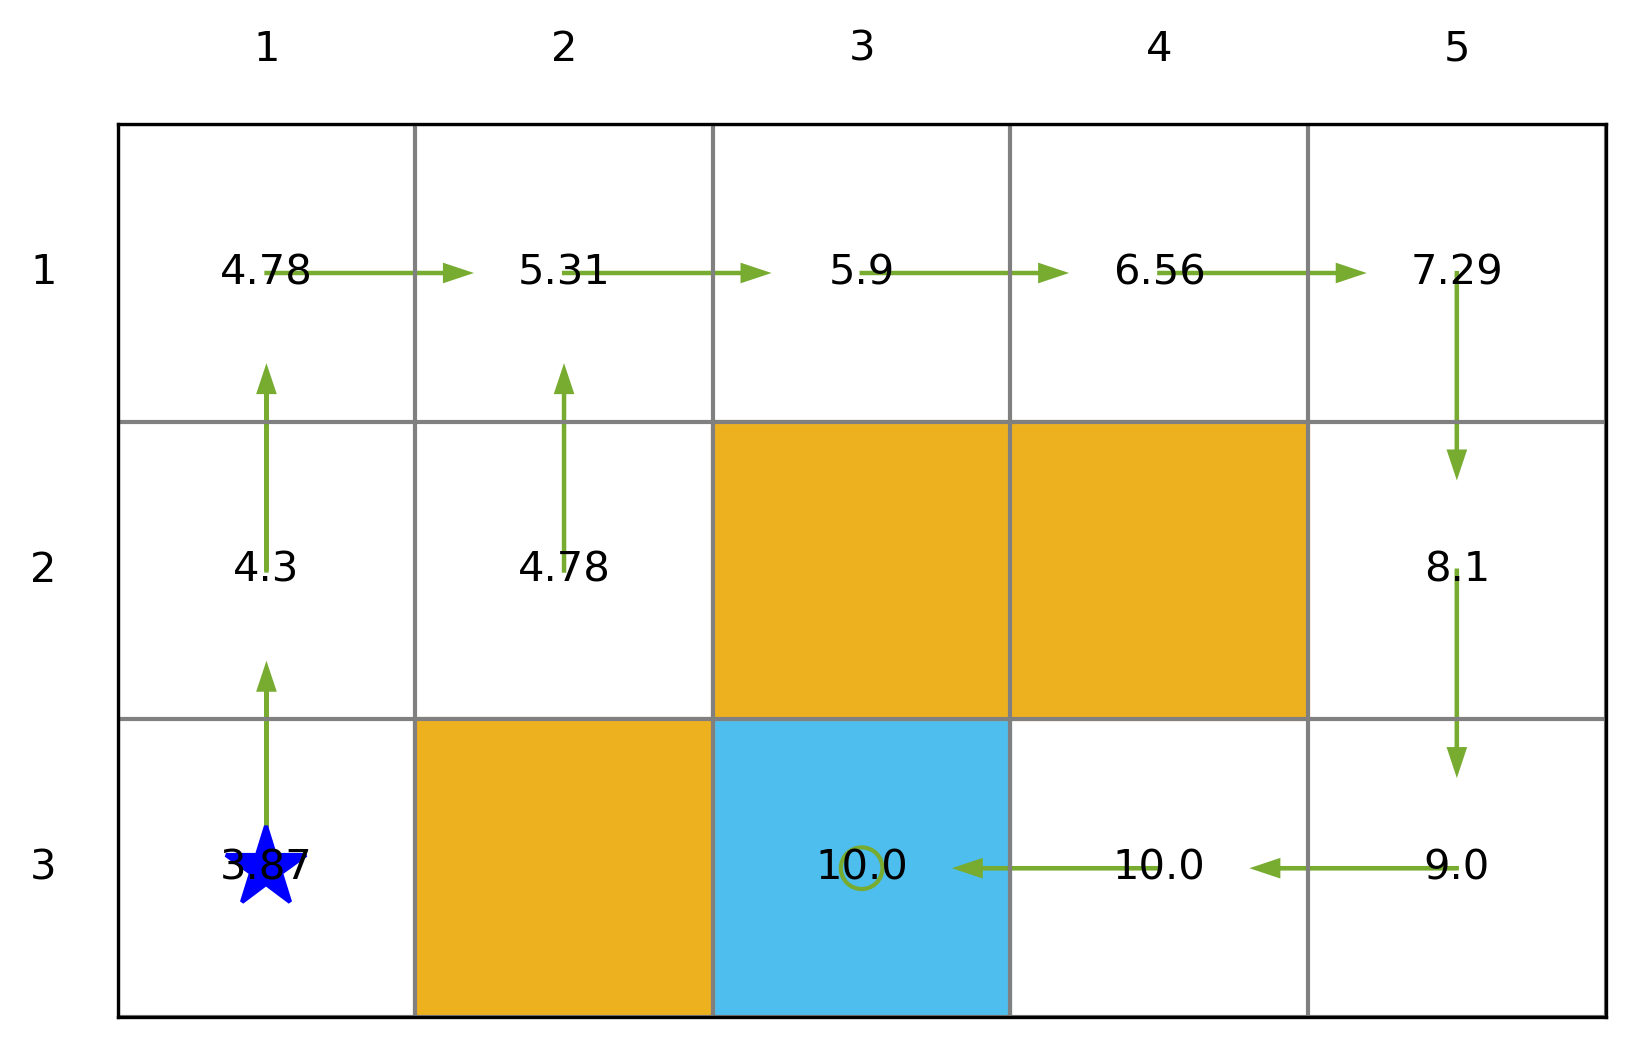
\includegraphics[width=0.8\textwidth]{output/deterministic_closed_form_values.png}
\caption{State values for the deterministic policy calculated via the closed-form method.}
\label{fig:det_closed}
\end{figure}

\subsection{Iterative Evaluation}
An alternative to the closed-form solution is iterative policy evaluation, which applies the Bellman update rule repeatedly until the value function converges:
\[ V^{(k+1)} = r^\pi + \gamma P^\pi V^{(k)} \]
This process is terminated when the maximum change between successive value functions, $\|V^{(k+1)} - V^{(k)}\|_\infty$, falls below a small tolerance. This method converged in 133 iterations. The final values, which match the closed-form solution, are shown below and plotted in Figure~\ref{fig:det_iter}.

\noindent\textbf{State Values $V^\pi$ (Iterative, 133 iterations):}
\begin{center}
\begin{tabular}{|c|c|c|c|c|c|c|c|c|c|c|c|c|}
\hline
\textbf{State} & S0 & S1 & S2 & S3 & S4 & S5 & S6 & S7 & S8 & S9 & S10 & S11 \\
\hline
\textbf{Value} & 4.78 & 4.30 & 3.87 & 5.31 & 4.78 & 5.90 & 10.0 & 6.56 & 10.0 & 7.29 & 8.1 & 9.0 \\
\hline
\end{tabular}
\end{center}

\begin{figure}[h!]
\centering
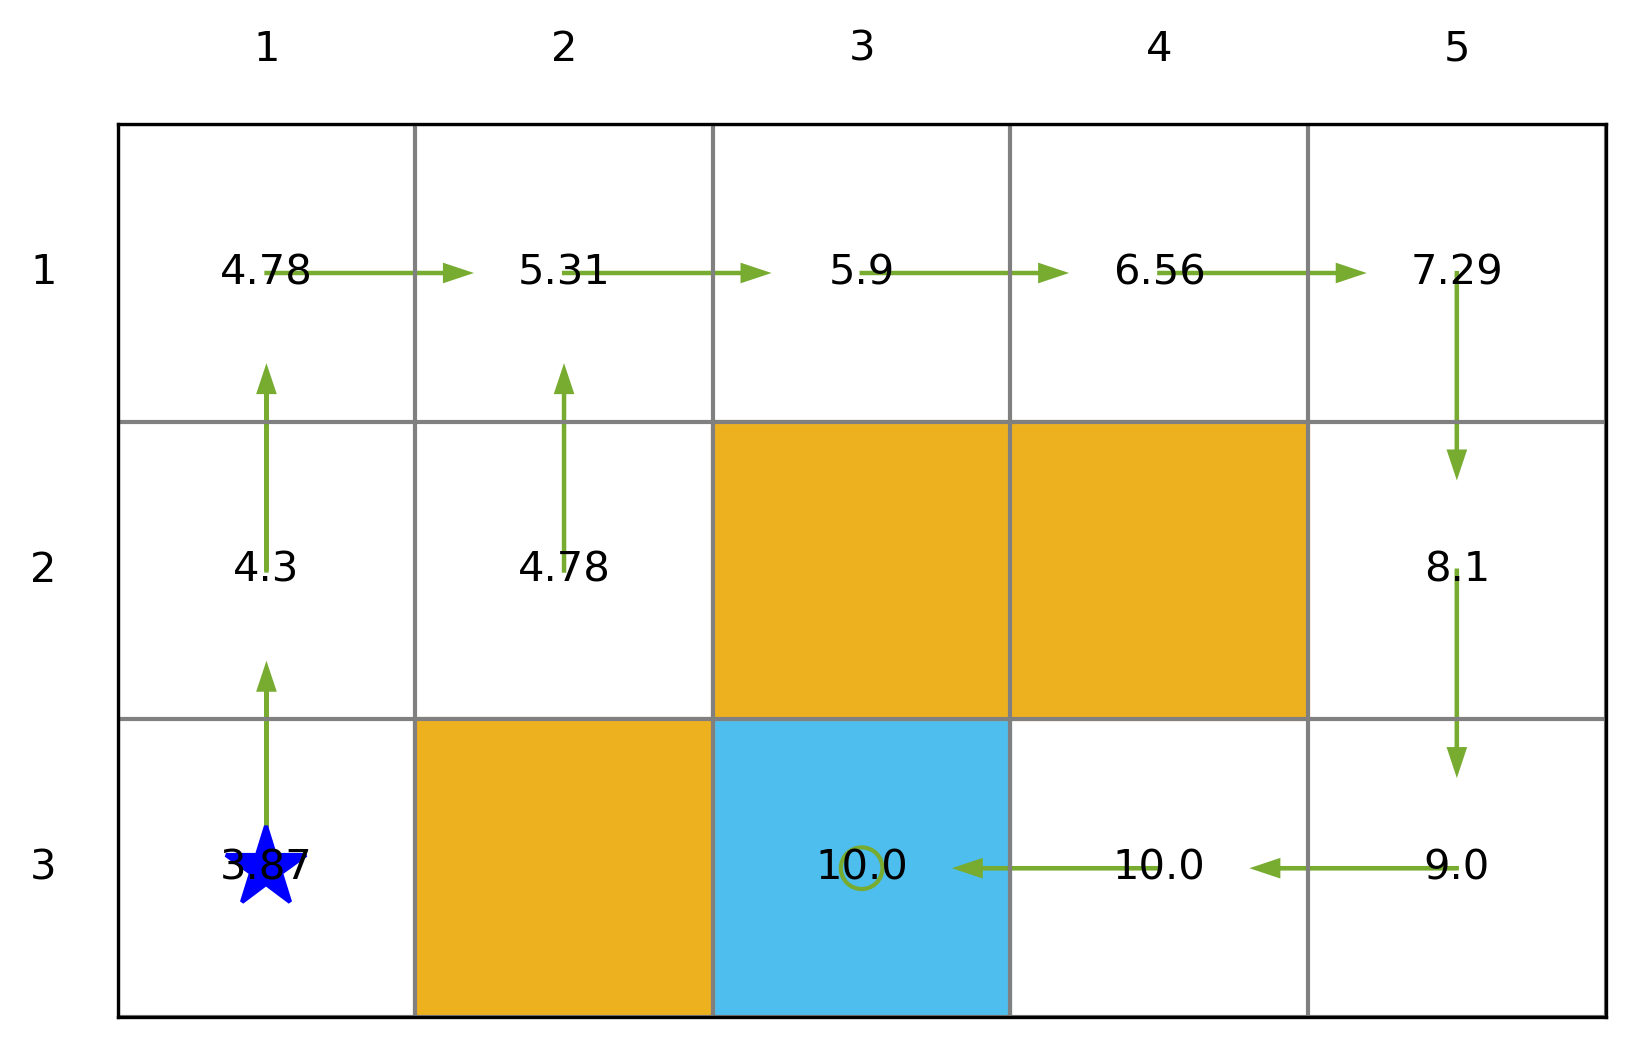
\includegraphics[width=0.8\textwidth]{output/deterministic_iterative_values.png}
\caption{State values for the deterministic policy calculated via the iterative method.}
\label{fig:det_iter}
\end{figure}

\newpage
\section{Policy 2: Stochastic Policy}
The second policy is stationary and stochastic. In non-terminal states, it selects actions based on a fixed probability distribution with a bias towards moving right (0.7), down/up (0.1 each), left (0.05), and stay (0.05).

\subsection{Policy Visualization}
Figure~\ref{fig:stoch_policy} illustrates the stochastic policy. The size of the arrows is proportional to the probability of taking that action in a given state.

\begin{figure}[h!]
\centering
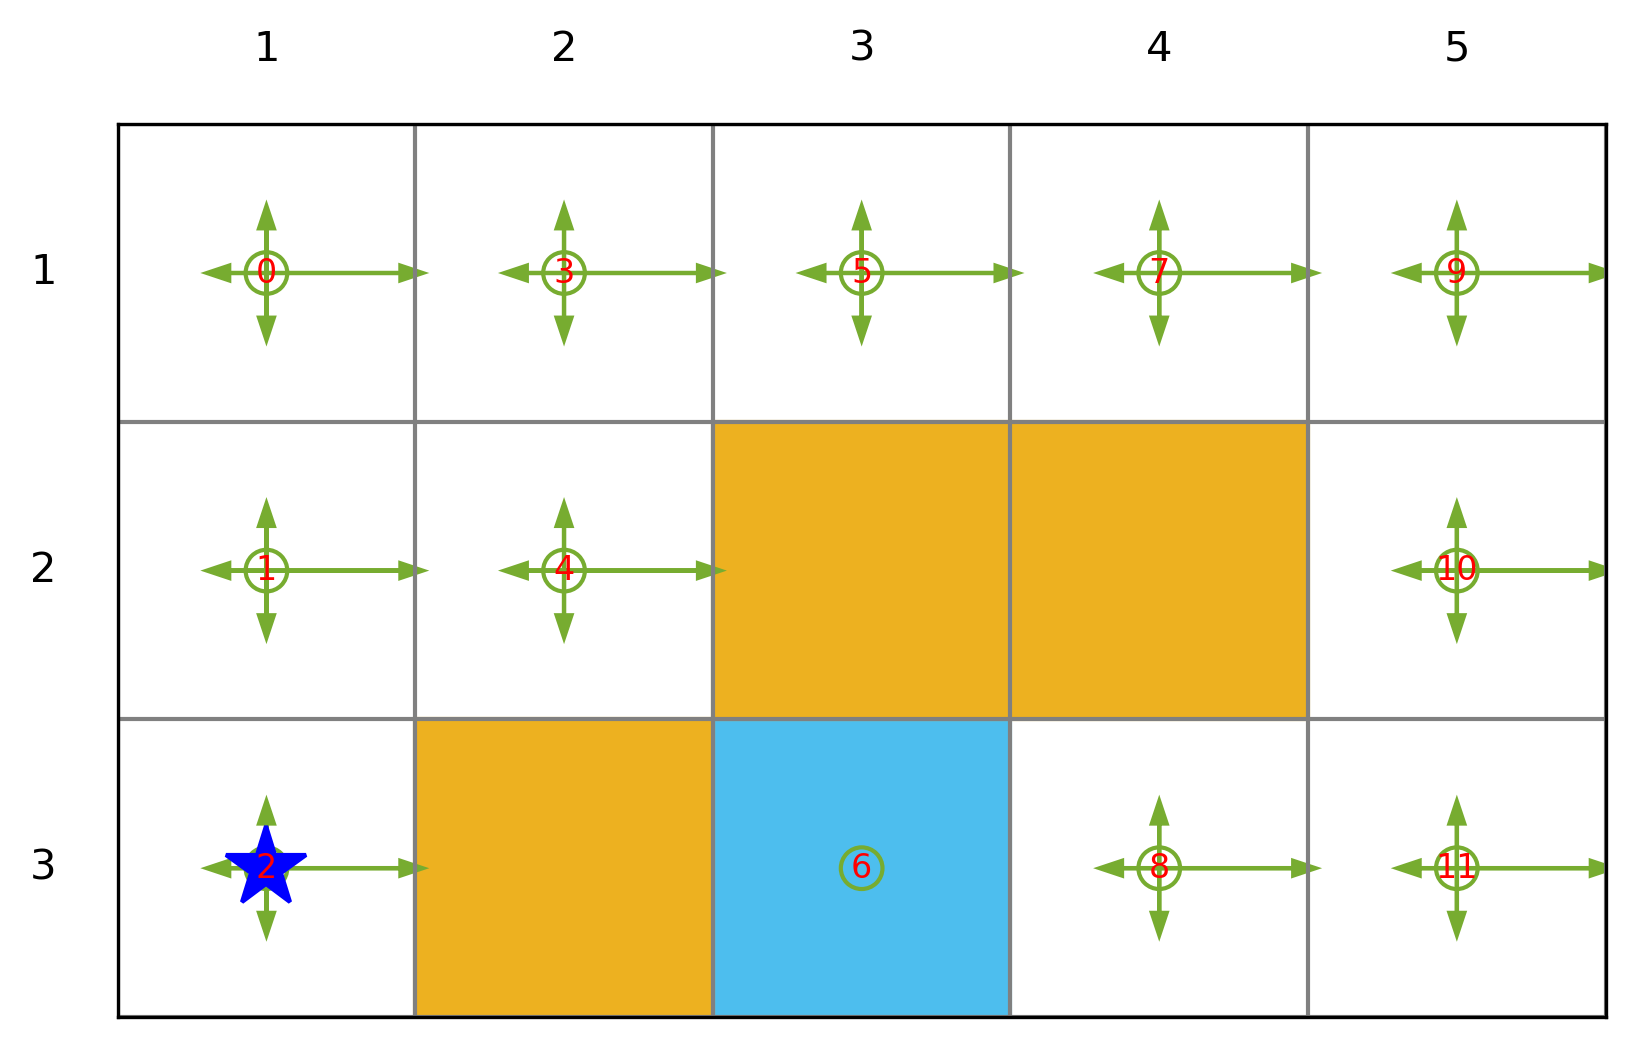
\includegraphics[width=0.8\textwidth]{output/stochastic_policy.png}
\caption{Stochastic policy visualized on the grid. Arrow size corresponds to action probability.}
\label{fig:stoch_policy}
\end{figure}

\subsection{Policy Dynamics: \texorpdfstring{$r^\pi$}{r pi} and \texorpdfstring{$P^\pi$}{P pi}}
The expected one-step rewards and transition probabilities for the stochastic policy are as follows.

\noindent\textbf{Reward Vector $r^\pi$:}

% Add a table to show the reward vector with state labels
\begin{center}
\begin{tabular}{|c|c|c|c|c|c|c|c|c|c|c|c|c|}
\hline
\textbf{State} & S0 & S1 & S2 & S3 & S4 & S5 & S6 & S7 & S8 & S9 & S10 & S11 \\
\hline
\textbf{Reward} & -0.15 & -0.05 & -0.85 & -0.1 & -0.8 & -0.2 & 1.0 & -0.2 & -0.15 & -0.8 & -0.75 & -0.8 \\
\hline
\end{tabular}
\end{center}

\noindent\textbf{Transition Matrix $P^\pi$:}

% Add a table to show the transition matrix with row and column labels
\begin{center}
\begin{tabular}{|c|c|c|c|c|c|c|c|c|c|c|c|c|c|}
\hline
\textbf{From/To} & \textbf{S0} & \textbf{S1} & \textbf{S2} & \textbf{S3} & \textbf{S4} & \textbf{S5} & \textbf{S6} & \textbf{S7} & \textbf{S8} & \textbf{S9} & \textbf{S10} & \textbf{S11} \\
\hline
\textbf{S0} & 0.2 & 0.1 & 0.0 & 0.7 & 0.0 & 0.0 & 0.0 & 0.0 & 0.0 & 0.0 & 0.0 & 0.0 \\
\hline
\textbf{S1} & 0.1 & 0.1 & 0.1 & 0.0 & 0.7 & 0.0 & 0.0 & 0.0 & 0.0 & 0.0 & 0.0 & 0.0 \\
\hline
\textbf{S2} & 0.0 & 0.1 & 0.9 & 0.0 & 0.0 & 0.0 & 0.0 & 0.0 & 0.0 & 0.0 & 0.0 & 0.0 \\
\hline
\textbf{S3} & 0.05 & 0.0 & 0.0 & 0.15 & 0.1 & 0.7 & 0.0 & 0.0 & 0.0 & 0.0 & 0.0 & 0.0 \\
\hline
\textbf{S4} & 0.0 & 0.05 & 0.0 & 0.1 & 0.85 & 0.0 & 0.0 & 0.0 & 0.0 & 0.0 & 0.0 & 0.0 \\
\hline
\textbf{S5} & 0.0 & 0.0 & 0.0 & 0.05 & 0.0 & 0.25 & 0.0 & 0.7 & 0.0 & 0.0 & 0.0 & 0.0 \\
\hline
\textbf{S6} & 0.0 & 0.0 & 0.0 & 0.0 & 0.0 & 0.0 & 1.0 & 0.0 & 0.0 & 0.0 & 0.0 & 0.0 \\
\hline
\textbf{S7} & 0.0 & 0.0 & 0.0 & 0.0 & 0.0 & 0.05 & 0.0 & 0.25 & 0.0 & 0.7 & 0.0 & 0.0 \\
\hline
\textbf{S8} & 0.0 & 0.0 & 0.0 & 0.0 & 0.0 & 0.0 & 0.05 & 0.0 & 0.25 & 0.0 & 0.0 & 0.7 \\
\hline
\textbf{S9} & 0.0 & 0.0 & 0.0 & 0.0 & 0.0 & 0.0 & 0.0 & 0.05 & 0.0 & 0.85 & 0.1 & 0.0 \\
\hline
\textbf{S10} & 0.0 & 0.0 & 0.0 & 0.0 & 0.0 & 0.0 & 0.0 & 0.0 & 0.0 & 0.1 & 0.8 & 0.1 \\
\hline
\textbf{S11} & 0.0 & 0.0 & 0.0 & 0.0 & 0.0 & 0.0 & 0.0 & 0.0 & 0.05 & 0.0 & 0.1 & 0.85 \\
\hline
\end{tabular}
\end{center}

\subsection{Closed-Form Evaluation}
Using the same direct solution method as before, we calculate the state values for the stochastic policy. The results are shown below and plotted in Figure~\ref{fig:stoch_closed}.

\noindent\textbf{State Values $V^\pi$ (Closed-Form):}
\begin{center}
\begin{tabular}{|c|c|c|c|c|c|c|c|c|c|c|c|c|}
\hline
\textbf{State} & S0 & S1 & S2 & S3 & S4 & S5 & S6 & S7 & S8 & S9 & S10 & S11 \\
\hline
\textbf{Value} & -5.04 & -5.86 & -7.25 & -5.48 & -6.63 & -6.07 & 10.0 & -6.75 & -5.57 & -7.56 & -7.46 & -7.33 \\
\hline
\end{tabular}
\end{center}

\begin{figure}[h!]
\centering
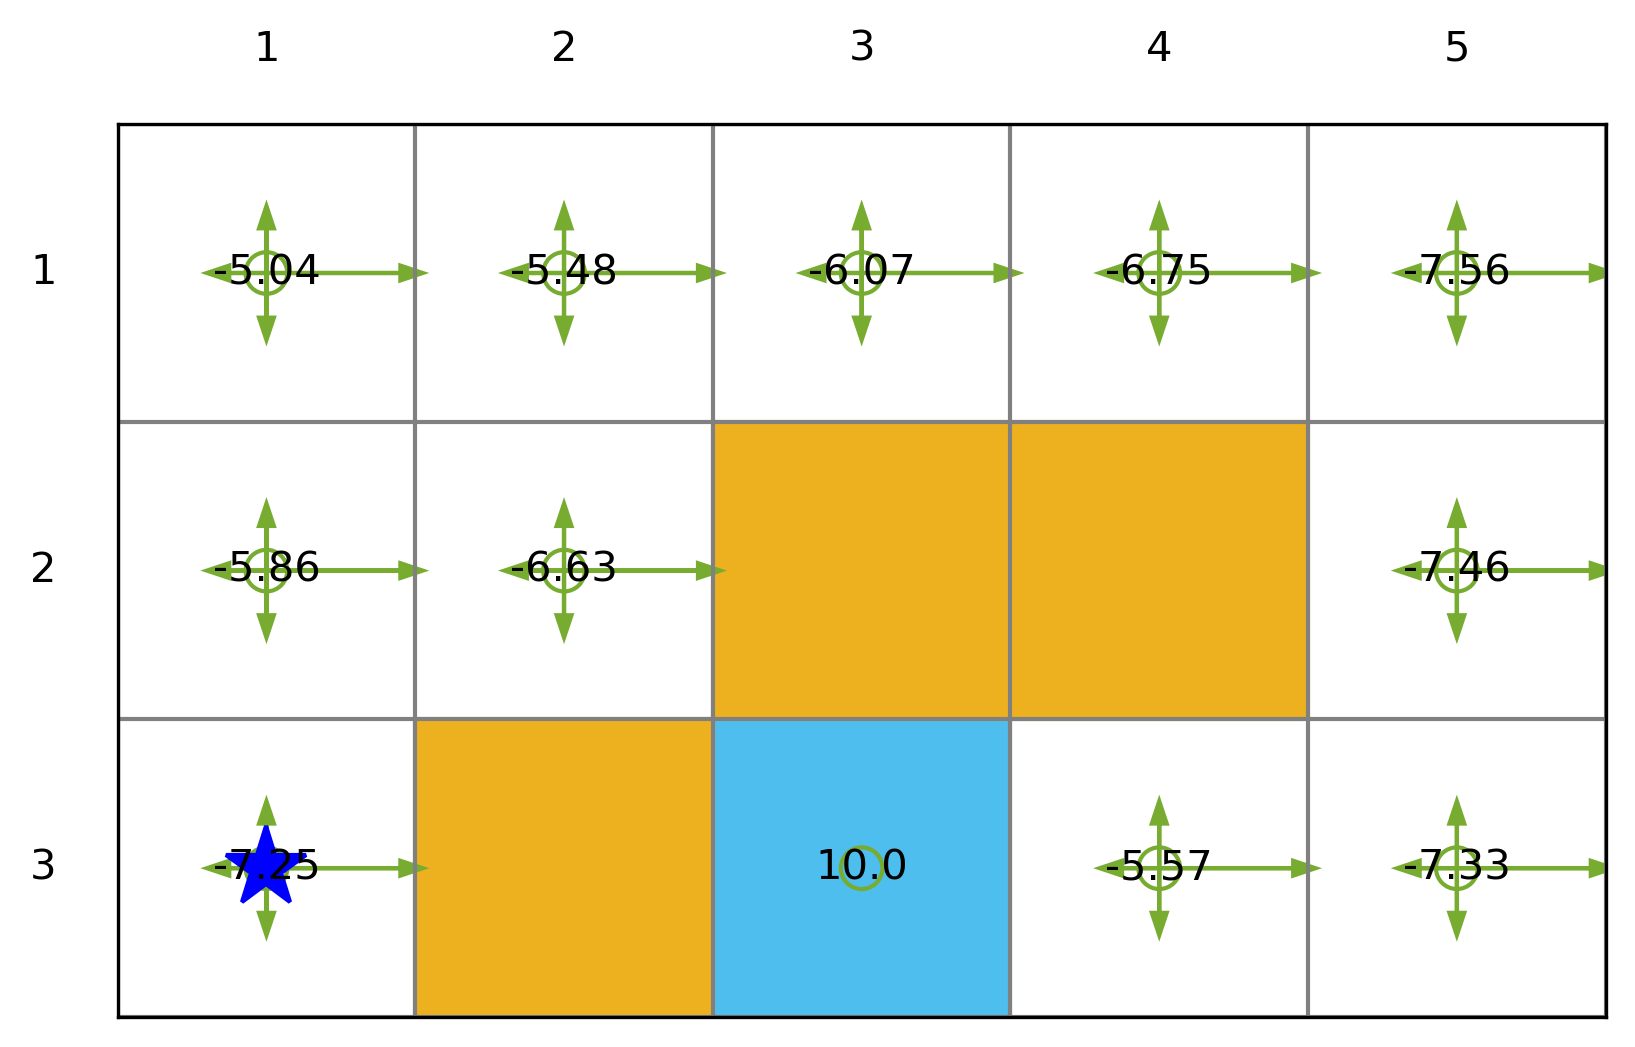
\includegraphics[width=0.8\textwidth]{output/stochastic_closed_form_values.png}
\caption{State values for the stochastic policy calculated via the closed-form method.}
\label{fig:stoch_closed}
\end{figure}

\subsection{Iterative Evaluation}
The iterative algorithm also converged in 133 iterations for the stochastic policy, yielding results consistent with the closed-form method. The values are presented below and in Figure~\ref{fig:stoch_iter}.

\noindent\textbf{State Values $V^\pi$ (Iterative, 133 iterations):}
\begin{center}
\begin{tabular}{|c|c|c|c|c|c|c|c|c|c|c|c|c|}
\hline
\textbf{State} & S0 & S1 & S2 & S3 & S4 & S5 & S6 & S7 & S8 & S9 & S10 & S11 \\
\hline
\textbf{Value} & -5.04 & -5.86 & -7.25 & -5.48 & -6.63 & -6.07 & 10.0 & -6.75 & -5.57 & -7.56 & -7.46 & -7.33 \\
\hline
\end{tabular}
\end{center}

\begin{figure}[h!]
\centering
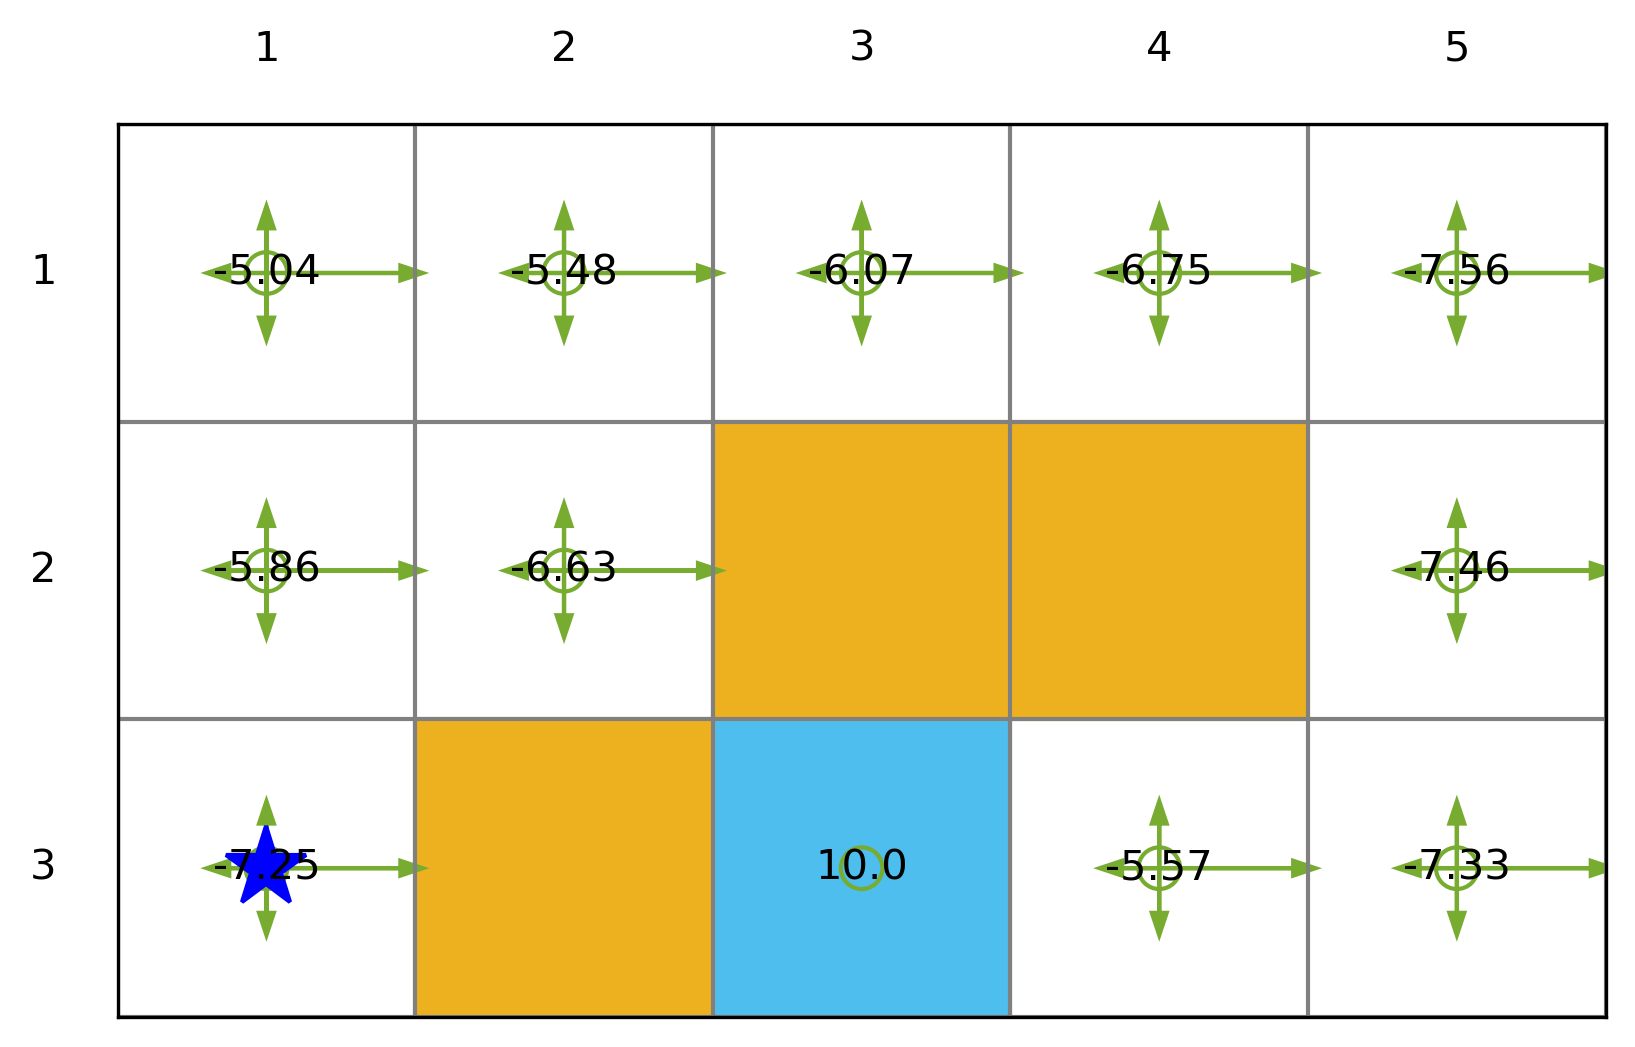
\includegraphics[width=0.8\textwidth]{output/stochastic_iterative_values.png}
\caption{State values for the stochastic policy calculated via the iterative method.}
\label{fig:stoch_iter}
\end{figure}

\newpage
\section{Discussion}
\textbf{Comparison of Policies:} The results clearly show the superiority of the deterministic, optimal policy. Its state values are all positive, increasing along the shortest paths toward the goal state, which has the maximum value of 10. This reflects the policy's effectiveness in reaching the target and accumulating rewards. In contrast, the stochastic policy performs poorly. Most of its state values are negative because its fixed action probabilities frequently lead the agent into forbidden states, incurring penalties. The negative values propagate throughout the state space, indicating that following this policy is generally undesirable.

\noindent\textbf{Comparison of Algorithms:} For both policies, the closed-form and iterative evaluation algorithms produced identical state values, as expected. The closed-form method provides an exact solution by solving a system of linear equations, which is feasible for this small state space. The iterative method converges to the same solution and is often more practical for larger state spaces where directly solving or inverting a large matrix would be computationally prohibitive. The number of iterations (133) shows a reasonably fast convergence for this problem.

\section{Key Code Implementation}
The core logic for policy evaluation is contained in the PolicyEvaluator class, which encapsulates the functionality for computing policy dynamics and evaluating state values using both closed-form and iterative methods.

\subsection{Deriving Policy Dynamics}
\label{sec:policy-dynamics}
This function computes the reward vector $r^\pi$ and transition matrix $P^\pi$ from the environment dynamics and a given policy matrix.
\begin{lstlisting}[language=Python, caption={Method to compute $r^\pi$ and $P^\pi$.}, label={lst:derive-policy-dynamics}]
def _derive_policy_markov_dynamics(self, world: GridWorld) -> Tuple[np.ndarray, np.ndarray]:
    """
    Compute r_pi and P_pi for a fixed policy:
       r_pi[s]     = E[R | s, a ~ pi(s)]
       P_pi[s,s']  = Pr(s' | s, a ~ pi(s)]
    """
    nS = world.num_states
    r_pi = np.zeros(nS, dtype=float)
    P_pi = np.zeros((nS, nS), dtype=float)

    acts = world.action_space
    s2i = world.state_to_idx
    i2s = world.idx_to_state

    # Accumulate expectation under action distribution
    for s in range(nS):
        xy = i2s[s]
        pmf = self.policy_matrix[s]
        if not np.any(pmf):
            continue
        for a_idx, prob in enumerate(pmf):
            if prob <= 0.0:
                continue
            nxt_xy, rew = world._get_next_state_and_reward(xy, acts[a_idx])
            s_next = s2i[nxt_xy]
            r_pi[s] += prob * rew
            P_pi[s, s_next] += prob

    return r_pi, P_pi
\end{lstlisting}

\subsection{Closed-Form Solution}
\label{sec:closed-form}
This function implements the direct, closed-form solution to the Bellman expectation equation.
\begin{lstlisting}[language=Python, caption={Function for closed-form policy evaluation.}, label={lst:closed-form-solution}]
def solve_analytically(self, gamma: float) -> np.ndarray:
    """
    Solve (I - gamma P)V = r via linear solve.
    """
    I = np.eye(self.transition_matrix.shape[0], dtype=float)
    return np.linalg.solve(I - gamma * self.transition_matrix, self.reward_vector)
\end{lstlisting}

\subsection{Iterative Solution}
\label{sec:iterative}
This function implements the iterative policy evaluation algorithm, which repeatedly applies the Bellman update until convergence.
\begin{lstlisting}[language=Python, caption={Function for iterative policy evaluation.}, label={lst:iterative-solution}]
def solve_iteratively(
    self,
    gamma: float,
    tol: float = 1e-6,
    max_iter: int = 10_000,
) -> Tuple[np.ndarray, int]:
    """
    Fixed-point iteration: V_{k+1} = r + gamma P V_k
    """
    v = np.zeros_like(self.reward_vector)
    for k in range(1, max_iter + 1):
        v_next = self.reward_vector + gamma * self.transition_matrix.dot(v)
        if np.max(np.abs(v_next - v)) < tol:
            return v_next, k
        v = v_next
    return v, max_iter
\end{lstlisting}

\subsection{Policy Creation}
\label{sec:policy-creation}
The deterministic and stochastic policies are created using dedicated functions that generate policy matrices.

\begin{lstlisting}[language=Python, caption={Deterministic policy creation using reverse BFS.}, label={lst:deterministic-policy}]
def create_optimal_path_policy(world: GridWorld) -> np.ndarray:
    """
    Build a deterministic policy by back-propagating shortest steps
    from the goal using a reverse BFS over the grid.
    """
    nS = world.num_states
    acts = world.action_space
    pi = np.zeros((nS, len(acts)), dtype=float)

    stay_idx = acts.index((0, 0))
    goal = tuple(world.target_state)

    # Reverse BFS: record a "next-hop" for each state toward the goal
    q = deque([goal])
    next_hop = {goal: None}

    H, W = world.env_size  # (rows, cols)

    while q:
        cur = q.popleft()
        # consider predecessors that could move into `cur`
        for dx, dy in acts:
            if dx == 0 and dy == 0:
                continue
            prev = (cur[0] - dx, cur[1] - dy)
            if 0 <= prev[0] < H and 0 <= prev[1] < W:
                if prev not in world.forbidden_states and prev not in next_hop:
                    next_hop[prev] = cur
                    q.append(prev)

    # Turn the shortest-next-hop map into a deterministic policy
    for s_idx in range(nS):
        s_xy = world.idx_to_state[s_idx]
        if s_xy == goal or s_xy in world.forbidden_states or s_xy not in next_hop:
            pi[s_idx, stay_idx] = 1.0
            continue

        nxt = next_hop[s_xy]
        move = (nxt[0] - s_xy[0], nxt[1] - s_xy[1])
        if move in acts:
            a_idx = acts.index(move)
            pi[s_idx, a_idx] = 1.0
        else:
            pi[s_idx, stay_idx] = 1.0

    return pi
\end{lstlisting}

\begin{lstlisting}[language=Python, caption={Stochastic policy creation with weighted actions.}, label={lst:stochastic-policy}]
def create_weighted_random_policy(world: GridWorld) -> np.ndarray:
    """
    Build a stationary stochastic policy with fixed action probabilities
    (except terminal/forbidden states that enforce 'stay').
    """
    nS = world.num_states
    acts = world.action_space
    pi = np.zeros((nS, len(acts)), dtype=float)

    # Weight mapping for stochastic policy
    _STOCH_WEIGHTS = {
        (1, 0): 0.7,    # right
        (0, 1): 0.1,    # down
        (0, -1): 0.1,   # up
        (-1, 0): 0.05,  # left
        (0, 0): 0.05    # stay
    }

    base = np.array([_STOCH_WEIGHTS.get(a, 0.0) for a in acts], dtype=float)
    base /= base.sum() if base.sum() > 0 else 1.0

    stay_idx = acts.index((0, 0))
    goal = tuple(world.target_state)

    for s_idx in range(nS):
        s_xy = world.idx_to_state[s_idx]
        if s_xy == goal or s_xy in world.forbidden_states:
            pi[s_idx, stay_idx] = 1.0
        else:
            pi[s_idx, :] = base

    return pi
\end{lstlisting}

\end{document}